\documentclass[1p]{elsarticle_modified}
%\bibliographystyle{elsarticle-num}

%\usepackage[colorlinks]{hyperref}
%\usepackage{abbrmath_seonhwa} %\Abb, \Ascr, \Acal ,\Abf, \Afrak
\usepackage{amsfonts}
\usepackage{amssymb}
\usepackage{amsmath}
\usepackage{amsthm}
\usepackage{scalefnt}
\usepackage{amsbsy}
\usepackage{kotex}
\usepackage{caption}
\usepackage{subfig}
\usepackage{color}
\usepackage{graphicx}
\usepackage{xcolor} %% white, black, red, green, blue, cyan, magenta, yellow
\usepackage{float}
\usepackage{setspace}
\usepackage{hyperref}

\usepackage{tikz}
\usetikzlibrary{arrows}

\usepackage{multirow}
\usepackage{array} % fixed length table
\usepackage{hhline}

%%%%%%%%%%%%%%%%%%%%%
\makeatletter
\renewcommand*\env@matrix[1][\arraystretch]{%
	\edef\arraystretch{#1}%
	\hskip -\arraycolsep
	\let\@ifnextchar\new@ifnextchar
	\array{*\c@MaxMatrixCols c}}
\makeatother %https://tex.stackexchange.com/questions/14071/how-can-i-increase-the-line-spacing-in-a-matrix
%%%%%%%%%%%%%%%

\usepackage[normalem]{ulem}

\newcommand{\msout}[1]{\ifmmode\text{\sout{\ensuremath{#1}}}\else\sout{#1}\fi}
%SOURCE: \msout is \stkout macro in https://tex.stackexchange.com/questions/20609/strikeout-in-math-mode

\newcommand{\cancel}[1]{
	\ifmmode
	{\color{red}\msout{#1}}
	\else
	{\color{red}\sout{#1}}
	\fi
}

\newcommand{\add}[1]{
	{\color{blue}\uwave{#1}}
}

\newcommand{\replace}[2]{
	\ifmmode
	{\color{red}\msout{#1}}{\color{blue}\uwave{#2}}
	\else
	{\color{red}\sout{#1}}{\color{blue}\uwave{#2}}
	\fi
}

\newcommand{\Sol}{\mathcal{S}} %segment
\newcommand{\D}{D} %diagram
\newcommand{\A}{\mathcal{A}} %arc


%%%%%%%%%%%%%%%%%%%%%%%%%%%%%5 test

\def\sl{\operatorname{\textup{SL}}(2,\Cbb)}
\def\psl{\operatorname{\textup{PSL}}(2,\Cbb)}
\def\quan{\mkern 1mu \triangleright \mkern 1mu}

\theoremstyle{definition}
\newtheorem{thm}{Theorem}[section]
\newtheorem{prop}[thm]{Proposition}
\newtheorem{lem}[thm]{Lemma}
\newtheorem{ques}[thm]{Question}
\newtheorem{cor}[thm]{Corollary}
\newtheorem{defn}[thm]{Definition}
\newtheorem{exam}[thm]{Example}
\newtheorem{rmk}[thm]{Remark}
\newtheorem{alg}[thm]{Algorithm}

\newcommand{\I}{\sqrt{-1}}
\begin{document}

%\begin{frontmatter}
%
%\title{Boundary parabolic representations of knots up to 8 crossings}
%
%%% Group authors per affiliation:
%\author{Yunhi Cho} 
%\address{Department of Mathematics, University of Seoul, Seoul, Korea}
%\ead{yhcho@uos.ac.kr}
%
%
%\author{Seonhwa Kim} %\fnref{s_kim}}
%\address{Center for Geometry and Physics, Institute for Basic Science, Pohang, 37673, Korea}
%\ead{ryeona17@ibs.re.kr}
%
%\author{Hyuk Kim}
%\address{Department of Mathematical Sciences, Seoul National University, Seoul 08826, Korea}
%\ead{hyukkim@snu.ac.kr}
%
%\author{Seokbeom Yoon}
%\address{Department of Mathematical Sciences, Seoul National University, Seoul, 08826,  Korea}
%\ead{sbyoon15@snu.ac.kr}
%
%\begin{abstract}
%We find all boundary parabolic representation of knots up to 8 crossings.
%
%\end{abstract}
%\begin{keyword}
%    \MSC[2010] 57M25 
%\end{keyword}
%
%\end{frontmatter}

%\linenumbers
%\tableofcontents
%
\newcommand\colored[1]{\textcolor{white}{\rule[-0.35ex]{0.8em}{1.4ex}}\kern-0.8em\color{red} #1}%
%\newcommand\colored[1]{\textcolor{white}{ #1}\kern-2.17ex	\textcolor{white}{ #1}\kern-1.81ex	\textcolor{white}{ #1}\kern-2.15ex\color{red}#1	}

{\Large $\underline{12n_{0604}~(K12n_{0604})}$}

\setlength{\tabcolsep}{10pt}
\renewcommand{\arraystretch}{1.6}
\vspace{1cm}\begin{tabular}{m{100pt}>{\centering\arraybackslash}m{274pt}}
\multirow{5}{120pt}{
	\centering
	\includegraphics[width=112pt]{../../../GIT/diagram.site/diagram/png/2693_12n_0604.png}\\
\ \ \ A knot diagram\footnotemark}&
\allowdisplaybreaks
\textbf{Linearized knot diagam} \\
\cline{2-2}
 &
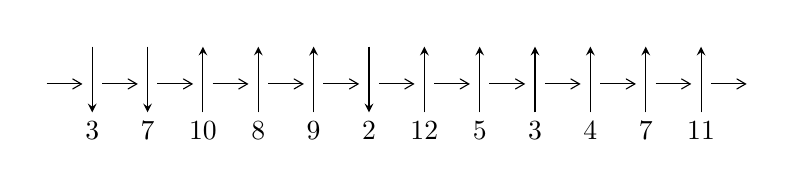
\begin{tikzpicture}[x=20pt, y=17pt]
	% nodes
	\node (C0) at (0, 0) {};
	\node (C1) at (1, 0) {};
	\node (C1U) at (1, +1) {};
	\node (C1D) at (1, -1) {3};

	\node (C2) at (2, 0) {};
	\node (C2U) at (2, +1) {};
	\node (C2D) at (2, -1) {7};

	\node (C3) at (3, 0) {};
	\node (C3U) at (3, +1) {};
	\node (C3D) at (3, -1) {10};

	\node (C4) at (4, 0) {};
	\node (C4U) at (4, +1) {};
	\node (C4D) at (4, -1) {8};

	\node (C5) at (5, 0) {};
	\node (C5U) at (5, +1) {};
	\node (C5D) at (5, -1) {9};

	\node (C6) at (6, 0) {};
	\node (C6U) at (6, +1) {};
	\node (C6D) at (6, -1) {2};

	\node (C7) at (7, 0) {};
	\node (C7U) at (7, +1) {};
	\node (C7D) at (7, -1) {12};

	\node (C8) at (8, 0) {};
	\node (C8U) at (8, +1) {};
	\node (C8D) at (8, -1) {5};

	\node (C9) at (9, 0) {};
	\node (C9U) at (9, +1) {};
	\node (C9D) at (9, -1) {3};

	\node (C10) at (10, 0) {};
	\node (C10U) at (10, +1) {};
	\node (C10D) at (10, -1) {4};

	\node (C11) at (11, 0) {};
	\node (C11U) at (11, +1) {};
	\node (C11D) at (11, -1) {7};

	\node (C12) at (12, 0) {};
	\node (C12U) at (12, +1) {};
	\node (C12D) at (12, -1) {11};
	\node (C13) at (13, 0) {};

	% arrows
	\draw[->,>={angle 60}]
	(C0) edge (C1) (C1) edge (C2) (C2) edge (C3) (C3) edge (C4) (C4) edge (C5) (C5) edge (C6) (C6) edge (C7) (C7) edge (C8) (C8) edge (C9) (C9) edge (C10) (C10) edge (C11) (C11) edge (C12) (C12) edge (C13) ;	\draw[->,>=stealth]
	(C1U) edge (C1D) (C2U) edge (C2D) (C3D) edge (C3U) (C4D) edge (C4U) (C5D) edge (C5U) (C6U) edge (C6D) (C7D) edge (C7U) (C8D) edge (C8U) (C9D) edge (C9U) (C10D) edge (C10U) (C11D) edge (C11U) (C12D) edge (C12U) ;
	\end{tikzpicture} \\
\hhline{~~} \\& 
\textbf{Solving Sequence} \\ \cline{2-2} 
 &
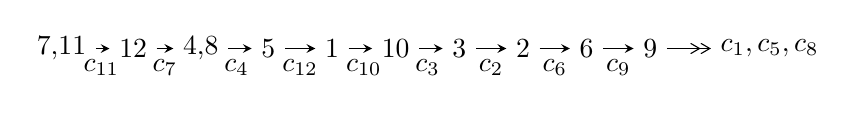
\begin{tikzpicture}[x=23pt, y=7pt]
	% node
	\node (A0) at (-1/8, 0) {7,11};
	\node (A1) at (1, 0) {12};
	\node (A2) at (33/16, 0) {4,8};
	\node (A3) at (25/8, 0) {5};
	\node (A4) at (33/8, 0) {1};
	\node (A5) at (41/8, 0) {10};
	\node (A6) at (49/8, 0) {3};
	\node (A7) at (57/8, 0) {2};
	\node (A8) at (65/8, 0) {6};
	\node (A9) at (73/8, 0) {9};
	\node (C1) at (1/2, -1) {$c_{11}$};
	\node (C2) at (3/2, -1) {$c_{7}$};
	\node (C3) at (21/8, -1) {$c_{4}$};
	\node (C4) at (29/8, -1) {$c_{12}$};
	\node (C5) at (37/8, -1) {$c_{10}$};
	\node (C6) at (45/8, -1) {$c_{3}$};
	\node (C7) at (53/8, -1) {$c_{2}$};
	\node (C8) at (61/8, -1) {$c_{6}$};
	\node (C9) at (69/8, -1) {$c_{9}$};
	\node (A10) at (11, 0) {$c_{1},c_{5},c_{8}$};

	% edge
	\draw[->,>=stealth]	
	(A0) edge (A1) (A1) edge (A2) (A2) edge (A3) (A3) edge (A4) (A4) edge (A5) (A5) edge (A6) (A6) edge (A7) (A7) edge (A8) (A8) edge (A9) ;
	\draw[->>,>={angle 60}]	
	(A9) edge (A10);
\end{tikzpicture} \\ 

\end{tabular} \\

\footnotetext{
The image of knot diagram is generated by the software ``\textbf{Draw programme}" developed by Andrew Bartholomew(\url{http://www.layer8.co.uk/maths/draw/index.htm\#Running-draw}), where we modified some parts for our purpose(\url{https://github.com/CATsTAILs/LinksPainter}).
}\phantom \\ \newline 
\centering \textbf{Ideals for irreducible components\footnotemark of $X_{\text{par}}$} 
 
\begin{align*}
I^u_{1}&=\langle 
6141 u^{12}+35469 u^{11}+\cdots+4348 b-14051,\;-17214 u^{12}-43917 u^{11}+\cdots+47828 a-232915,\\
\phantom{I^u_{1}}&\phantom{= \langle  }3 u^{13}+18 u^{12}+47 u^{11}+60 u^{10}+14 u^9-84 u^8-153 u^7-114 u^6+14 u^5+105 u^4+80 u^3+2 u^2-25 u-11\rangle \\
I^u_{2}&=\langle 
u^9-2 u^8+u^7+2 u^6-2 u^5- u^4+u^2 a+3 u^3- a u+b-2 u+1,\;-2 u^{10} a-13 u^{10}+\cdots-2 a-35,\\
\phantom{I^u_{2}}&\phantom{= \langle  }u^{11}-2 u^{10}+4 u^8-2 u^7-4 u^6+5 u^5+2 u^4-5 u^3+u^2+3 u-1\rangle \\
I^u_{3}&=\langle 
b+2 a+1,\;2 a^2+2 a-1,\;u-1\rangle \\
I^u_{4}&=\langle 
-2 a u+2 b-2 a+u+3,\;4 a^2-4 a+1,\;u^2+2 u+1\rangle \\
I^u_{5}&=\langle 
b,\;a-1,\;u^3- u+1\rangle \\
I^u_{6}&=\langle 
b+1,\;a+u,\;u^3- u+1\rangle \\
I^u_{7}&=\langle 
b,\;a-1,\;u-1\rangle \\
I^u_{8}&=\langle 
b+1,\;u^2 a- a u-1\rangle \\
I^u_{9}&=\langle 
b+1,\;u+1\rangle \\
\\
\end{align*}
\raggedright * 7 irreducible components of $\dim_{\mathbb{C}}=0$, with total 48 representations.\\
\raggedright * 2 irreducible components of $\dim_{\mathbb{C}}=1$ \\
\footnotetext{All coefficients of polynomials are rational numbers. But the coefficients are sometimes approximated in decimal forms when there is not enough margin.}
\newpage
\renewcommand{\arraystretch}{1}
\centering \section*{I. $I^u_{1}= \langle 6141 u^{12}+35469 u^{11}+\cdots+4348 b-14051,\;-1.72\times10^{4} u^{12}-4.39\times10^{4} u^{11}+\cdots+4.78\times10^{4} a-2.33\times10^{5},\;3 u^{13}+18 u^{12}+\cdots-25 u-11 \rangle$}
\flushleft \textbf{(i) Arc colorings}\\
\begin{tabular}{m{7pt} m{180pt} m{7pt} m{180pt} }
\flushright $a_{7}=$&$\begin{pmatrix}0\\u\end{pmatrix}$ \\
\flushright $a_{11}=$&$\begin{pmatrix}1\\0\end{pmatrix}$ \\
\flushright $a_{12}=$&$\begin{pmatrix}1\\- u^2\end{pmatrix}$ \\
\flushright $a_{4}=$&$\begin{pmatrix}0.359915 u^{12}+0.918228 u^{11}+\cdots+7.51984 u+4.86985\\-1.41237 u^{12}-8.15754 u^{11}+\cdots+1.15501 u+3.23160\end{pmatrix}$ \\
\flushright $a_{8}=$&$\begin{pmatrix}u\\- u^3+u\end{pmatrix}$ \\
\flushright $a_{5}=$&$\begin{pmatrix}0.676612 u^{12}+3.37246 u^{11}+\cdots-1.01834 u-0.308857\\1.52001 u^{12}+5.01127 u^{11}+\cdots-13.1615 u-3.97861\end{pmatrix}$ \\
\flushright $a_{1}=$&$\begin{pmatrix}- u^2+1\\- u^2\end{pmatrix}$ \\
\flushright $a_{10}=$&$\begin{pmatrix}-1.17283 u^{12}-6.60021 u^{11}+\cdots-6.76142 u-0.483336\\0.411914 u^{12}+3.59407 u^{11}+\cdots+11.9177 u+2.69894\end{pmatrix}$ \\
\flushright $a_{3}=$&$\begin{pmatrix}-0.863344 u^{12}-5.14142 u^{11}+\cdots-4.86443 u+1.08965\\-0.00965961 u^{12}+1.66697 u^{11}+\cdots+20.0262 u+7.04140\end{pmatrix}$ \\
\flushright $a_{2}=$&$\begin{pmatrix}-0.863344 u^{12}-5.14142 u^{11}+\cdots-4.86443 u+1.08965\\0.890064 u^{12}+5.82889 u^{11}+\cdots+22.8698 u+6.89972\end{pmatrix}$ \\
\flushright $a_{6}=$&$\begin{pmatrix}0.234089 u^{12}+2.30426 u^{11}+\cdots+5.28669 u+0.892866\\-0.449862 u^{12}-3.58096 u^{11}+\cdots-21.4218 u-6.42916\end{pmatrix}$ \\
\flushright $a_{9}=$&$\begin{pmatrix}0.0502425 u^{12}+0.933470 u^{11}+\cdots+1.62986 u-0.0270135\\0.638224 u^{12}+1.82498 u^{11}+\cdots-21.8395 u-8.12810\end{pmatrix}$\\&\end{tabular}
\flushleft \textbf{(ii) Obstruction class $= -1$}\\~\\
\flushleft \textbf{(iii) Cusp Shapes $= -\frac{9825}{2174} u^{12}-\frac{54711}{2174} u^{11}+\cdots-\frac{20596}{1087} u+\frac{3441}{2174}$}\\~\\
\newpage\renewcommand{\arraystretch}{1}
\flushleft \textbf{(iv) u-Polynomials at the component}\newline \\
\begin{tabular}{m{50pt}|m{274pt}}
Crossings & \hspace{64pt}u-Polynomials at each crossing \\
\hline $$\begin{aligned}c_{1}\end{aligned}$$&$\begin{aligned}
&9(9 u^{13}+114 u^{12}+\cdots+1485 u+121)
\end{aligned}$\\
\hline $$\begin{aligned}c_{2},c_{6}\end{aligned}$$&$\begin{aligned}
&3(3 u^{13}-18 u^{12}+\cdots+11 u-11)
\end{aligned}$\\
\hline $$\begin{aligned}c_{3},c_{4},c_{5}\\c_{8},c_{9},c_{10}\end{aligned}$$&$\begin{aligned}
&u^{13}+2 u^{12}+\cdots-2 u+2
\end{aligned}$\\
\hline $$\begin{aligned}c_{7},c_{11}\end{aligned}$$&$\begin{aligned}
&3(3 u^{13}+18 u^{12}+\cdots-25 u-11)
\end{aligned}$\\
\hline $$\begin{aligned}c_{12}\end{aligned}$$&$\begin{aligned}
&9(9 u^{13}-42 u^{12}+\cdots+669 u-121)
\end{aligned}$\\
\hline
\end{tabular}\\~\\
\newpage\renewcommand{\arraystretch}{1}
\flushleft \textbf{(v) Riley Polynomials at the component}\newline \\
\begin{tabular}{m{50pt}|m{274pt}}
Crossings & \hspace{64pt}Riley Polynomials at each crossing \\
\hline $$\begin{aligned}c_{1}\end{aligned}$$&$\begin{aligned}
&81(81 y^{13}-1962 y^{12}+\cdots+662717 y-14641)
\end{aligned}$\\
\hline $$\begin{aligned}c_{2},c_{6}\end{aligned}$$&$\begin{aligned}
&9(9 y^{13}-114 y^{12}+\cdots+1485 y-121)
\end{aligned}$\\
\hline $$\begin{aligned}c_{3},c_{4},c_{5}\\c_{8},c_{9},c_{10}\end{aligned}$$&$\begin{aligned}
&y^{13}-12 y^{12}+\cdots+16 y-4
\end{aligned}$\\
\hline $$\begin{aligned}c_{7},c_{11}\end{aligned}$$&$\begin{aligned}
&9(9 y^{13}-42 y^{12}+\cdots+669 y-121)
\end{aligned}$\\
\hline $$\begin{aligned}c_{12}\end{aligned}$$&$\begin{aligned}
&81(81 y^{13}+630 y^{12}+\cdots+37613 y-14641)
\end{aligned}$\\
\hline
\end{tabular}\\~\\
\newpage\flushleft \textbf{(vi) Complex Volumes and Cusp Shapes}
$$\begin{array}{c|c|c}  
\text{Solutions to }I^u_{1}& \I (\text{vol} + \sqrt{-1}CS) & \text{Cusp shape}\\
 \hline 
\begin{aligned}
u &= \phantom{-}1.15461\phantom{ +0.000000I} \\
a &= -0.667204\phantom{ +0.000000I} \\
b &= \phantom{-}1.65982\phantom{ +0.000000I}\end{aligned}
 & \phantom{-}14.2281\phantom{ +0.000000I} & \phantom{-}19.7580\phantom{ +0.000000I} \\ \hline\begin{aligned}
u &= -0.875852 + 0.854559 I \\
a &= -0.480641 - 0.877360 I \\
b &= \phantom{-}0.160333 - 1.044863 I\end{aligned}
 & -8.47998 - 3.13363 I & \phantom{-}2.30766 + 3.10183 I \\ \hline\begin{aligned}
u &= -0.875852 - 0.854559 I \\
a &= -0.480641 + 0.877360 I \\
b &= \phantom{-}0.160333 + 1.044863 I\end{aligned}
 & -8.47998 + 3.13363 I & \phantom{-}2.30766 - 3.10183 I \\ \hline\begin{aligned}
u &= -0.195045 + 1.209339 I \\
a &= \phantom{-}0.484703 + 0.539351 I \\
b &= \phantom{-}1.182797 + 0.515971 I\end{aligned}
 & -2.29018 + 7.80194 I & \phantom{-}7.00595 - 5.86285 I \\ \hline\begin{aligned}
u &= -0.195045 - 1.209339 I \\
a &= \phantom{-}0.484703 - 0.539351 I \\
b &= \phantom{-}1.182797 - 0.515971 I\end{aligned}
 & -2.29018 - 7.80194 I & \phantom{-}7.00595 + 5.86285 I \\ \hline\begin{aligned}
u &= -0.602765 + 0.436556 I \\
a &= \phantom{-}0.289714 + 1.181214 I \\
b &= \phantom{-}0.018598 + 0.533941 I\end{aligned}
 & -0.98838 - 1.46599 I & \phantom{-}1.41277 + 4.35204 I \\ \hline\begin{aligned}
u &= -0.602765 - 0.436556 I \\
a &= \phantom{-}0.289714 - 1.181214 I \\
b &= \phantom{-}0.018598 - 0.533941 I\end{aligned}
 & -0.98838 + 1.46599 I & \phantom{-}1.41277 - 4.35204 I \\ \hline\begin{aligned}
u &= \phantom{-}0.734365\phantom{ +0.000000I} \\
a &= \phantom{-}0.253961\phantom{ +0.000000I} \\
b &= -0.323459\phantom{ +0.000000I}\end{aligned}
 & \phantom{-}0.880574\phantom{ +0.000000I} & \phantom{-}13.4560\phantom{ +0.000000I} \\ \hline\begin{aligned}
u &= \phantom{-}0.692816\phantom{ +0.000000I} \\
a &= \phantom{-}1.53700\phantom{ +0.000000I} \\
b &= -1.80261\phantom{ +0.000000I}\end{aligned}
 & \phantom{-}12.2154\phantom{ +0.000000I} & \phantom{-}2.46050\phantom{ +0.000000I} \\ \hline\begin{aligned}
u &= -1.32583 + 0.68048 I \\
a &= \phantom{-}0.433863 + 1.256459 I \\
b &= -1.39870 + 0.52665 I\end{aligned}
 & \phantom{-}1.1831 - 14.4275 I & \phantom{-}9.59825 + 7.66969 I\\
 \hline 
 \end{array}$$\newpage$$\begin{array}{c|c|c}  
\text{Solutions to }I^u_{1}& \I (\text{vol} + \sqrt{-1}CS) & \text{Cusp shape}\\
 \hline 
\begin{aligned}
u &= -1.32583 - 0.68048 I \\
a &= \phantom{-}0.433863 - 1.256459 I \\
b &= -1.39870 - 0.52665 I\end{aligned}
 & \phantom{-}1.1831 + 14.4275 I & \phantom{-}9.59825 - 7.66969 I \\ \hline\begin{aligned}
u &= -1.29140 + 0.76843 I \\
a &= -0.107698 - 1.063230 I \\
b &= \phantom{-}1.270099 - 0.358705 I\end{aligned}
 & \phantom{-}6.78301 - 8.58406 I & \phantom{-}12.8385 + 7.0528 I \\ \hline\begin{aligned}
u &= -1.29140 - 0.76843 I \\
a &= -0.107698 + 1.063230 I \\
b &= \phantom{-}1.270099 + 0.358705 I\end{aligned}
 & \phantom{-}6.78301 + 8.58406 I & \phantom{-}12.8385 - 7.0528 I\\
 \hline 
 \end{array}$$\newpage\newpage\renewcommand{\arraystretch}{1}
\centering \section*{II. $I^u_{2}= \langle u^9-2 u^8+\cdots+b+1,\;-2 u^{10} a-13 u^{10}+\cdots-2 a-35,\;u^{11}-2 u^{10}+\cdots+3 u-1 \rangle$}
\flushleft \textbf{(i) Arc colorings}\\
\begin{tabular}{m{7pt} m{180pt} m{7pt} m{180pt} }
\flushright $a_{7}=$&$\begin{pmatrix}0\\u\end{pmatrix}$ \\
\flushright $a_{11}=$&$\begin{pmatrix}1\\0\end{pmatrix}$ \\
\flushright $a_{12}=$&$\begin{pmatrix}1\\- u^2\end{pmatrix}$ \\
\flushright $a_{4}=$&$\begin{pmatrix}a\\- u^9+2 u^8- u^7-2 u^6+2 u^5+u^4- u^2 a-3 u^3+a u+2 u-1\end{pmatrix}$ \\
\flushright $a_{8}=$&$\begin{pmatrix}u\\- u^3+u\end{pmatrix}$ \\
\flushright $a_{5}=$&$\begin{pmatrix}- u^9+2 u^8-3 u^6+2 u^5+u^3 a+2 u^4- u^2 a-3 u^3+a+3 u-1\\-2 u^9+3 u^8+\cdots+2 u-1\end{pmatrix}$ \\
\flushright $a_{1}=$&$\begin{pmatrix}- u^2+1\\- u^2\end{pmatrix}$ \\
\flushright $a_{10}=$&$\begin{pmatrix}- u^{10} a+u^{10}+\cdots- u+5\\- u^8 a+u^7 a- u^5 a- u^2 a+u^3- u^2+1\end{pmatrix}$ \\
\flushright $a_{3}=$&$\begin{pmatrix}u^{10}-2 u^9- u^8+5 u^7- u^6-6 u^5+4 u^4+4 u^3-5 u^2- u+3\\u^{10}-2 u^9- u^8+4 u^7- u^6-4 u^5+2 u^4+2 u^3-3 u^2- u+1\end{pmatrix}$ \\
\flushright $a_{2}=$&$\begin{pmatrix}u^{10}-2 u^9- u^8+5 u^7- u^6-6 u^5+4 u^4+4 u^3-5 u^2- u+3\\2 u^{10}-3 u^9-2 u^8+6 u^7-6 u^5+2 u^4+4 u^3-3 u^2-2 u+1\end{pmatrix}$ \\
\flushright $a_{6}=$&$\begin{pmatrix}u^{10}- u^9- u^8+3 u^7-3 u^5+3 u^4+2 u^3-3 u^2+2\\- u^{10}+u^9+3 u^8-3 u^7-4 u^6+7 u^5+2 u^4-6 u^3+2 u^2+4 u-1\end{pmatrix}$ \\
\flushright $a_{9}=$&$\begin{pmatrix}u^{10}- u^9+\cdots+a+4\\u^{10} a- u^9 a+\cdots+a+1\end{pmatrix}$\\&\end{tabular}
\flushleft \textbf{(ii) Obstruction class $= -1$}\\~\\
\flushleft \textbf{(iii) Cusp Shapes $= -4 u^{10}+6 u^9-10 u^7+4 u^6+6 u^5-12 u^4-4 u^3+8 u^2-6 u+4$}\\~\\
\newpage\renewcommand{\arraystretch}{1}
\flushleft \textbf{(iv) u-Polynomials at the component}\newline \\
\begin{tabular}{m{50pt}|m{274pt}}
Crossings & \hspace{64pt}u-Polynomials at each crossing \\
\hline $$\begin{aligned}c_{1}\end{aligned}$$&$\begin{aligned}
&(u^{11}+12 u^{10}+\cdots-5 u+1)^{2}
\end{aligned}$\\
\hline $$\begin{aligned}c_{2},c_{6}\end{aligned}$$&$\begin{aligned}
&(u^{11}+2 u^{10}-4 u^9-8 u^8+6 u^7+8 u^6-7 u^5+2 u^4+7 u^3-3 u^2- u-1)^2
\end{aligned}$\\
\hline $$\begin{aligned}c_{3},c_{4},c_{5}\\c_{8},c_{9},c_{10}\end{aligned}$$&$\begin{aligned}
&u^{22}+2 u^{21}+\cdots-54 u-23
\end{aligned}$\\
\hline $$\begin{aligned}c_{7},c_{11}\end{aligned}$$&$\begin{aligned}
&(u^{11}-2 u^{10}+4 u^8-2 u^7-4 u^6+5 u^5+2 u^4-5 u^3+u^2+3 u-1)^2
\end{aligned}$\\
\hline $$\begin{aligned}c_{12}\end{aligned}$$&$\begin{aligned}
&(u^{11}-4 u^{10}+\cdots+11 u-1)^{2}
\end{aligned}$\\
\hline
\end{tabular}\\~\\
\newpage\renewcommand{\arraystretch}{1}
\flushleft \textbf{(v) Riley Polynomials at the component}\newline \\
\begin{tabular}{m{50pt}|m{274pt}}
Crossings & \hspace{64pt}Riley Polynomials at each crossing \\
\hline $$\begin{aligned}c_{1}\end{aligned}$$&$\begin{aligned}
&(y^{11}-24 y^{10}+\cdots-13 y-1)^{2}
\end{aligned}$\\
\hline $$\begin{aligned}c_{2},c_{6}\end{aligned}$$&$\begin{aligned}
&(y^{11}-12 y^{10}+\cdots-5 y-1)^{2}
\end{aligned}$\\
\hline $$\begin{aligned}c_{3},c_{4},c_{5}\\c_{8},c_{9},c_{10}\end{aligned}$$&$\begin{aligned}
&y^{22}-16 y^{21}+\cdots-1306 y+529
\end{aligned}$\\
\hline $$\begin{aligned}c_{7},c_{11}\end{aligned}$$&$\begin{aligned}
&(y^{11}-4 y^{10}+\cdots+11 y-1)^{2}
\end{aligned}$\\
\hline $$\begin{aligned}c_{12}\end{aligned}$$&$\begin{aligned}
&(y^{11}+8 y^{10}+\cdots+67 y-1)^{2}
\end{aligned}$\\
\hline
\end{tabular}\\~\\
\newpage\flushleft \textbf{(vi) Complex Volumes and Cusp Shapes}
$$\begin{array}{c|c|c}  
\text{Solutions to }I^u_{2}& \I (\text{vol} + \sqrt{-1}CS) & \text{Cusp shape}\\
 \hline 
\begin{aligned}
u &= -0.952018 + 0.226513 I \\
a &= -0.347172 - 0.939025 I \\
b &= -0.930670 - 0.421418 I\end{aligned}
 & \phantom{-}5.02081 - 0.74196 I & \phantom{-}15.5393 + 1.1191 I \\ \hline\begin{aligned}
u &= -0.952018 + 0.226513 I \\
a &= -1.36874 - 1.45440 I \\
b &= \phantom{-}1.254363 - 0.162092 I\end{aligned}
 & \phantom{-}5.02081 - 0.74196 I & \phantom{-}15.5393 + 1.1191 I \\ \hline\begin{aligned}
u &= -0.952018 - 0.226513 I \\
a &= -0.347172 + 0.939025 I \\
b &= -0.930670 + 0.421418 I\end{aligned}
 & \phantom{-}5.02081 + 0.74196 I & \phantom{-}15.5393 - 1.1191 I \\ \hline\begin{aligned}
u &= -0.952018 - 0.226513 I \\
a &= -1.36874 + 1.45440 I \\
b &= \phantom{-}1.254363 + 0.162092 I\end{aligned}
 & \phantom{-}5.02081 + 0.74196 I & \phantom{-}15.5393 - 1.1191 I \\ \hline\begin{aligned}
u &= -0.850023 + 0.614930 I \\
a &= \phantom{-}0.76372 + 1.33350 I \\
b &= -1.49337 + 0.42695 I\end{aligned}
 & \phantom{-}0.08426 - 2.41892 I & \phantom{-}7.07184 + 2.88947 I \\ \hline\begin{aligned}
u &= -0.850023 + 0.614930 I \\
a &= \phantom{-}0.077370 + 0.159281 I \\
b &= \phantom{-}1.27603 + 0.68990 I\end{aligned}
 & \phantom{-}0.08426 - 2.41892 I & \phantom{-}7.07184 + 2.88947 I \\ \hline\begin{aligned}
u &= -0.850023 - 0.614930 I \\
a &= \phantom{-}0.76372 - 1.33350 I \\
b &= -1.49337 - 0.42695 I\end{aligned}
 & \phantom{-}0.08426 + 2.41892 I & \phantom{-}7.07184 - 2.88947 I \\ \hline\begin{aligned}
u &= -0.850023 - 0.614930 I \\
a &= \phantom{-}0.077370 - 0.159281 I \\
b &= \phantom{-}1.27603 - 0.68990 I\end{aligned}
 & \phantom{-}0.08426 + 2.41892 I & \phantom{-}7.07184 - 2.88947 I \\ \hline\begin{aligned}
u &= \phantom{-}0.523691 + 0.948055 I \\
a &= -0.534548 + 1.013410 I \\
b &= \phantom{-}0.196709 + 0.952827 I\end{aligned}
 & -5.32590 - 2.58451 I & \phantom{-}3.80806 + 1.01660 I \\ \hline\begin{aligned}
u &= \phantom{-}0.523691 + 0.948055 I \\
a &= \phantom{-}0.382826 - 0.290327 I \\
b &= \phantom{-}1.191516 - 0.585396 I\end{aligned}
 & -5.32590 - 2.58451 I & \phantom{-}3.80806 + 1.01660 I\\
 \hline 
 \end{array}$$\newpage$$\begin{array}{c|c|c}  
\text{Solutions to }I^u_{2}& \I (\text{vol} + \sqrt{-1}CS) & \text{Cusp shape}\\
 \hline 
\begin{aligned}
u &= \phantom{-}0.523691 - 0.948055 I \\
a &= -0.534548 - 1.013410 I \\
b &= \phantom{-}0.196709 - 0.952827 I\end{aligned}
 & -5.32590 + 2.58451 I & \phantom{-}3.80806 - 1.01660 I \\ \hline\begin{aligned}
u &= \phantom{-}0.523691 - 0.948055 I \\
a &= \phantom{-}0.382826 + 0.290327 I \\
b &= \phantom{-}1.191516 + 0.585396 I\end{aligned}
 & -5.32590 + 2.58451 I & \phantom{-}3.80806 - 1.01660 I \\ \hline\begin{aligned}
u &= \phantom{-}0.978643 + 0.595733 I \\
a &= -0.010571 - 0.992888 I \\
b &= -0.109176 - 0.710565 I\end{aligned}
 & \phantom{-}2.61864 + 4.69742 I & \phantom{-}9.08124 - 5.88322 I \\ \hline\begin{aligned}
u &= \phantom{-}0.978643 + 0.595733 I \\
a &= -0.17727 + 1.45820 I \\
b &= \phantom{-}1.225999 + 0.305614 I\end{aligned}
 & \phantom{-}2.61864 + 4.69742 I & \phantom{-}9.08124 - 5.88322 I \\ \hline\begin{aligned}
u &= \phantom{-}0.978643 - 0.595733 I \\
a &= -0.010571 + 0.992888 I \\
b &= -0.109176 + 0.710565 I\end{aligned}
 & \phantom{-}2.61864 - 4.69742 I & \phantom{-}9.08124 + 5.88322 I \\ \hline\begin{aligned}
u &= \phantom{-}0.978643 - 0.595733 I \\
a &= -0.17727 - 1.45820 I \\
b &= \phantom{-}1.225999 - 0.305614 I\end{aligned}
 & \phantom{-}2.61864 - 4.69742 I & \phantom{-}9.08124 + 5.88322 I \\ \hline\begin{aligned}
u &= \phantom{-}1.126055 + 0.711355 I \\
a &= -0.407610 + 0.813195 I \\
b &= \phantom{-}0.097811 + 1.107042 I\end{aligned}
 & -3.47965 + 8.65115 I & \phantom{-}6.21430 - 5.57892 I \\ \hline\begin{aligned}
u &= \phantom{-}1.126055 + 0.711355 I \\
a &= \phantom{-}0.531471 - 1.289216 I \\
b &= -1.43289 - 0.49484 I\end{aligned}
 & -3.47965 + 8.65115 I & \phantom{-}6.21430 - 5.57892 I \\ \hline\begin{aligned}
u &= \phantom{-}1.126055 - 0.711355 I \\
a &= -0.407610 - 0.813195 I \\
b &= \phantom{-}0.097811 - 1.107042 I\end{aligned}
 & -3.47965 - 8.65115 I & \phantom{-}6.21430 + 5.57892 I \\ \hline\begin{aligned}
u &= \phantom{-}1.126055 - 0.711355 I \\
a &= \phantom{-}0.531471 + 1.289216 I \\
b &= -1.43289 + 0.49484 I\end{aligned}
 & -3.47965 - 8.65115 I & \phantom{-}6.21430 + 5.57892 I\\
 \hline 
 \end{array}$$\newpage$$\begin{array}{c|c|c}  
\text{Solutions to }I^u_{2}& \I (\text{vol} + \sqrt{-1}CS) & \text{Cusp shape}\\
 \hline 
\begin{aligned}
u &= \phantom{-}0.347303\phantom{ +0.000000I} \\
a &= -3.28286\phantom{ +0.000000I} \\
b &= -1.15435\phantom{ +0.000000I}\end{aligned}
 & \phantom{-}2.16369\phantom{ +0.000000I} & \phantom{-}2.57060\phantom{ +0.000000I} \\ \hline\begin{aligned}
u &= \phantom{-}0.347303\phantom{ +0.000000I} \\
a &= \phantom{-}4.46391\phantom{ +0.000000I} \\
b &= \phantom{-}0.601712\phantom{ +0.000000I}\end{aligned}
 & \phantom{-}2.16369\phantom{ +0.000000I} & \phantom{-}2.57060\phantom{ +0.000000I}\\
 \hline 
 \end{array}$$\newpage\newpage\renewcommand{\arraystretch}{1}
\centering \section*{III. $I^u_{3}= \langle b+2 a+1,\;2 a^2+2 a-1,\;u-1 \rangle$}
\flushleft \textbf{(i) Arc colorings}\\
\begin{tabular}{m{7pt} m{180pt} m{7pt} m{180pt} }
\flushright $a_{7}=$&$\begin{pmatrix}0\\1\end{pmatrix}$ \\
\flushright $a_{11}=$&$\begin{pmatrix}1\\0\end{pmatrix}$ \\
\flushright $a_{12}=$&$\begin{pmatrix}1\\-1\end{pmatrix}$ \\
\flushright $a_{4}=$&$\begin{pmatrix}a\\-2 a-1\end{pmatrix}$ \\
\flushright $a_{8}=$&$\begin{pmatrix}1\\0\end{pmatrix}$ \\
\flushright $a_{5}=$&$\begin{pmatrix}- a-1\\-2 a-1\end{pmatrix}$ \\
\flushright $a_{1}=$&$\begin{pmatrix}0\\-1\end{pmatrix}$ \\
\flushright $a_{10}=$&$\begin{pmatrix}a\\3\end{pmatrix}$ \\
\flushright $a_{3}=$&$\begin{pmatrix}1\\4 a+2\end{pmatrix}$ \\
\flushright $a_{2}=$&$\begin{pmatrix}1\\4 a+1\end{pmatrix}$ \\
\flushright $a_{6}=$&$\begin{pmatrix}1\\4 a+2\end{pmatrix}$ \\
\flushright $a_{9}=$&$\begin{pmatrix}- a-1\\-3\end{pmatrix}$\\&\end{tabular}
\flushleft \textbf{(ii) Obstruction class $= 1$}\\~\\
\flushleft \textbf{(iii) Cusp Shapes $= 12$}\\~\\
\newpage\renewcommand{\arraystretch}{1}
\flushleft \textbf{(iv) u-Polynomials at the component}\newline \\
\begin{tabular}{m{50pt}|m{274pt}}
Crossings & \hspace{64pt}u-Polynomials at each crossing \\
\hline $$\begin{aligned}c_{1},c_{2},c_{11}\\c_{12}\end{aligned}$$&$\begin{aligned}
&(u-1)^2
\end{aligned}$\\
\hline $$\begin{aligned}c_{3},c_{4},c_{5}\\c_{8},c_{9},c_{10}\end{aligned}$$&$\begin{aligned}
&u^2-3
\end{aligned}$\\
\hline $$\begin{aligned}c_{6},c_{7}\end{aligned}$$&$\begin{aligned}
&(u+1)^2
\end{aligned}$\\
\hline
\end{tabular}\\~\\
\newpage\renewcommand{\arraystretch}{1}
\flushleft \textbf{(v) Riley Polynomials at the component}\newline \\
\begin{tabular}{m{50pt}|m{274pt}}
Crossings & \hspace{64pt}Riley Polynomials at each crossing \\
\hline $$\begin{aligned}c_{1},c_{2},c_{6}\\c_{7},c_{11},c_{12}\end{aligned}$$&$\begin{aligned}
&(y-1)^2
\end{aligned}$\\
\hline $$\begin{aligned}c_{3},c_{4},c_{5}\\c_{8},c_{9},c_{10}\end{aligned}$$&$\begin{aligned}
&(y-3)^2
\end{aligned}$\\
\hline
\end{tabular}\\~\\
\newpage\flushleft \textbf{(vi) Complex Volumes and Cusp Shapes}
$$\begin{array}{c|c|c}  
\text{Solutions to }I^u_{3}& \I (\text{vol} + \sqrt{-1}CS) & \text{Cusp shape}\\
 \hline 
\begin{aligned}
u &= \phantom{-}1.00000\phantom{ +0.000000I} \\
a &= -1.36603\phantom{ +0.000000I} \\
b &= \phantom{-}1.73205\phantom{ +0.000000I}\end{aligned}
 & \phantom{-}13.1595\phantom{ +0.000000I} & \phantom{-}12.0000\phantom{ +0.000000I} \\ \hline\begin{aligned}
u &= \phantom{-}1.00000\phantom{ +0.000000I} \\
a &= \phantom{-}0.366025\phantom{ +0.000000I} \\
b &= -1.73205\phantom{ +0.000000I}\end{aligned}
 & \phantom{-}13.1595\phantom{ +0.000000I} & \phantom{-}12.0000\phantom{ +0.000000I}\\
 \hline 
 \end{array}$$\newpage\newpage\renewcommand{\arraystretch}{1}
\centering \section*{IV. $I^u_{4}= \langle -2 a u+2 b-2 a+u+3,\;4 a^2-4 a+1,\;u^2+2 u+1 \rangle$}
\flushleft \textbf{(i) Arc colorings}\\
\begin{tabular}{m{7pt} m{180pt} m{7pt} m{180pt} }
\flushright $a_{7}=$&$\begin{pmatrix}0\\u\end{pmatrix}$ \\
\flushright $a_{11}=$&$\begin{pmatrix}1\\0\end{pmatrix}$ \\
\flushright $a_{12}=$&$\begin{pmatrix}1\\2 u+1\end{pmatrix}$ \\
\flushright $a_{4}=$&$\begin{pmatrix}a\\a u+a-\frac{1}{2} u-\frac{3}{2}\end{pmatrix}$ \\
\flushright $a_{8}=$&$\begin{pmatrix}u\\-2 u-2\end{pmatrix}$ \\
\flushright $a_{5}=$&$\begin{pmatrix}- a u+\frac{3}{2} u+\frac{1}{2}\\a u+a-\frac{5}{2} u-\frac{7}{2}\end{pmatrix}$ \\
\flushright $a_{1}=$&$\begin{pmatrix}2 u+2\\2 u+1\end{pmatrix}$ \\
\flushright $a_{10}=$&$\begin{pmatrix}\frac{1}{2} a u-\frac{1}{2} a-\frac{1}{4} u+\frac{3}{4}\\-2 a u-2 a+u+2\end{pmatrix}$ \\
\flushright $a_{3}=$&$\begin{pmatrix}1\\-2 a u-2 a+u+1\end{pmatrix}$ \\
\flushright $a_{2}=$&$\begin{pmatrix}1\\-2 a u-2 a+3 u+2\end{pmatrix}$ \\
\flushright $a_{6}=$&$\begin{pmatrix}u\\2 a u+2 a-3 u-3\end{pmatrix}$ \\
\flushright $a_{9}=$&$\begin{pmatrix}\frac{3}{2} a u+\frac{1}{2} a-\frac{3}{4} u-\frac{3}{4}\\1\end{pmatrix}$\\&\end{tabular}
\flushleft \textbf{(ii) Obstruction class $= 1$}\\~\\
\flushleft \textbf{(iii) Cusp Shapes $= 12$}\\~\\
\newpage\renewcommand{\arraystretch}{1}
\flushleft \textbf{(iv) u-Polynomials at the component}\newline \\
\begin{tabular}{m{50pt}|m{274pt}}
Crossings & \hspace{64pt}u-Polynomials at each crossing \\
\hline $$\begin{aligned}c_{1},c_{3},c_{6}\\c_{7},c_{8},c_{12}\end{aligned}$$&$\begin{aligned}
&(u-1)^4
\end{aligned}$\\
\hline $$\begin{aligned}c_{2},c_{4},c_{5}\\c_{9},c_{10},c_{11}\end{aligned}$$&$\begin{aligned}
&(u+1)^4
\end{aligned}$\\
\hline
\end{tabular}\\~\\
\newpage\renewcommand{\arraystretch}{1}
\flushleft \textbf{(v) Riley Polynomials at the component}\newline \\
\begin{tabular}{m{50pt}|m{274pt}}
Crossings & \hspace{64pt}Riley Polynomials at each crossing \\
\hline $$\begin{aligned}c_{1},c_{2},c_{3}\\c_{4},c_{5},c_{6}\\c_{7},c_{8},c_{9}\\c_{10},c_{11},c_{12}\end{aligned}$$&$\begin{aligned}
&(y-1)^4
\end{aligned}$\\
\hline
\end{tabular}\\~\\
\newpage\flushleft \textbf{(vi) Complex Volumes and Cusp Shapes}
$$\begin{array}{c|c|c}  
\text{Solutions to }I^u_{4}& \I (\text{vol} + \sqrt{-1}CS) & \text{Cusp shape}\\
 \hline 
\begin{aligned}
u &= -1.00000\phantom{ +0.000000I} \\
a &= \phantom{-}0.500000\phantom{ +0.000000I} \\
b &= -1.00000\phantom{ +0.000000I}\end{aligned}
 & \phantom{-}3.28987\phantom{ +0.000000I} & \phantom{-}12.0000\phantom{ +0.000000I} \\ \hline\begin{aligned}
u &= -1.00000\phantom{ +0.000000I} \\
a &= \phantom{-}0.500000\phantom{ +0.000000I} \\
b &= -1.00000\phantom{ +0.000000I}\end{aligned}
 & \phantom{-}3.28987\phantom{ +0.000000I} & \phantom{-}12.0000\phantom{ +0.000000I} \\ \hline\begin{aligned}
u &= -1.00000\phantom{ +0.000000I} \\
a &= \phantom{-}0.500000\phantom{ +0.000000I} \\
b &= -1.00000\phantom{ +0.000000I}\end{aligned}
 & \phantom{-}3.28987\phantom{ +0.000000I} & \phantom{-}12.0000\phantom{ +0.000000I} \\ \hline\begin{aligned}
u &= -1.00000\phantom{ +0.000000I} \\
a &= \phantom{-}0.500000\phantom{ +0.000000I} \\
b &= -1.00000\phantom{ +0.000000I}\end{aligned}
 & \phantom{-}3.28987\phantom{ +0.000000I} & \phantom{-}12.0000\phantom{ +0.000000I}\\
 \hline 
 \end{array}$$\newpage\newpage\renewcommand{\arraystretch}{1}
\centering \section*{V. $I^u_{5}= \langle b,\;a-1,\;u^3- u+1 \rangle$}
\flushleft \textbf{(i) Arc colorings}\\
\begin{tabular}{m{7pt} m{180pt} m{7pt} m{180pt} }
\flushright $a_{7}=$&$\begin{pmatrix}0\\u\end{pmatrix}$ \\
\flushright $a_{11}=$&$\begin{pmatrix}1\\0\end{pmatrix}$ \\
\flushright $a_{12}=$&$\begin{pmatrix}1\\- u^2\end{pmatrix}$ \\
\flushright $a_{4}=$&$\begin{pmatrix}1\\0\end{pmatrix}$ \\
\flushright $a_{8}=$&$\begin{pmatrix}u\\1\end{pmatrix}$ \\
\flushright $a_{5}=$&$\begin{pmatrix}- u+1\\-1\end{pmatrix}$ \\
\flushright $a_{1}=$&$\begin{pmatrix}- u^2+1\\- u^2\end{pmatrix}$ \\
\flushright $a_{10}=$&$\begin{pmatrix}1\\0\end{pmatrix}$ \\
\flushright $a_{3}=$&$\begin{pmatrix}1\\0\end{pmatrix}$ \\
\flushright $a_{2}=$&$\begin{pmatrix}1\\- u^2\end{pmatrix}$ \\
\flushright $a_{6}=$&$\begin{pmatrix}u\\1\end{pmatrix}$ \\
\flushright $a_{9}=$&$\begin{pmatrix}1\\0\end{pmatrix}$\\&\end{tabular}
\flushleft \textbf{(ii) Obstruction class $= -1$}\\~\\
\flushleft \textbf{(iii) Cusp Shapes $= 6$}\\~\\
\newpage\renewcommand{\arraystretch}{1}
\flushleft \textbf{(iv) u-Polynomials at the component}\newline \\
\begin{tabular}{m{50pt}|m{274pt}}
Crossings & \hspace{64pt}u-Polynomials at each crossing \\
\hline $$\begin{aligned}c_{1}\end{aligned}$$&$\begin{aligned}
&u^3+2 u^2+u+1
\end{aligned}$\\
\hline $$\begin{aligned}c_{2},c_{6},c_{7}\\c_{11}\end{aligned}$$&$\begin{aligned}
&u^3- u+1
\end{aligned}$\\
\hline $$\begin{aligned}c_{3},c_{9},c_{10}\end{aligned}$$&$\begin{aligned}
&u^3
\end{aligned}$\\
\hline $$\begin{aligned}c_{4},c_{5},c_{8}\end{aligned}$$&$\begin{aligned}
&(u-1)^3
\end{aligned}$\\
\hline $$\begin{aligned}c_{12}\end{aligned}$$&$\begin{aligned}
&u^3-2 u^2+u-1
\end{aligned}$\\
\hline
\end{tabular}\\~\\
\newpage\renewcommand{\arraystretch}{1}
\flushleft \textbf{(v) Riley Polynomials at the component}\newline \\
\begin{tabular}{m{50pt}|m{274pt}}
Crossings & \hspace{64pt}Riley Polynomials at each crossing \\
\hline $$\begin{aligned}c_{1},c_{12}\end{aligned}$$&$\begin{aligned}
&y^3-2 y^2-3 y-1
\end{aligned}$\\
\hline $$\begin{aligned}c_{2},c_{6},c_{7}\\c_{11}\end{aligned}$$&$\begin{aligned}
&y^3-2 y^2+y-1
\end{aligned}$\\
\hline $$\begin{aligned}c_{3},c_{9},c_{10}\end{aligned}$$&$\begin{aligned}
&y^3
\end{aligned}$\\
\hline $$\begin{aligned}c_{4},c_{5},c_{8}\end{aligned}$$&$\begin{aligned}
&(y-1)^3
\end{aligned}$\\
\hline
\end{tabular}\\~\\
\newpage\flushleft \textbf{(vi) Complex Volumes and Cusp Shapes}
$$\begin{array}{c|c|c}  
\text{Solutions to }I^u_{5}& \I (\text{vol} + \sqrt{-1}CS) & \text{Cusp shape}\\
 \hline 
\begin{aligned}
u &= \phantom{-}0.662359 + 0.562280 I \\
a &= \phantom{-}1.00000\phantom{ +0.000000I} \\
b &= \phantom{-0.000000 } 0\end{aligned}
 & \phantom{-}1.64493\phantom{ +0.000000I} & \phantom{-}6.00000\phantom{ +0.000000I} \\ \hline\begin{aligned}
u &= \phantom{-}0.662359 - 0.562280 I \\
a &= \phantom{-}1.00000\phantom{ +0.000000I} \\
b &= \phantom{-0.000000 } 0\end{aligned}
 & \phantom{-}1.64493\phantom{ +0.000000I} & \phantom{-}6.00000\phantom{ +0.000000I} \\ \hline\begin{aligned}
u &= -1.32472\phantom{ +0.000000I} \\
a &= \phantom{-}1.00000\phantom{ +0.000000I} \\
b &= \phantom{-0.000000 } 0\end{aligned}
 & \phantom{-}1.64493\phantom{ +0.000000I} & \phantom{-}6.00000\phantom{ +0.000000I}\\
 \hline 
 \end{array}$$\newpage\newpage\renewcommand{\arraystretch}{1}
\centering \section*{VI. $I^u_{6}= \langle b+1,\;a+u,\;u^3- u+1 \rangle$}
\flushleft \textbf{(i) Arc colorings}\\
\begin{tabular}{m{7pt} m{180pt} m{7pt} m{180pt} }
\flushright $a_{7}=$&$\begin{pmatrix}0\\u\end{pmatrix}$ \\
\flushright $a_{11}=$&$\begin{pmatrix}1\\0\end{pmatrix}$ \\
\flushright $a_{12}=$&$\begin{pmatrix}1\\- u^2\end{pmatrix}$ \\
\flushright $a_{4}=$&$\begin{pmatrix}- u\\-1\end{pmatrix}$ \\
\flushright $a_{8}=$&$\begin{pmatrix}u\\1\end{pmatrix}$ \\
\flushright $a_{5}=$&$\begin{pmatrix}- u\\-1\end{pmatrix}$ \\
\flushright $a_{1}=$&$\begin{pmatrix}- u^2+1\\- u^2\end{pmatrix}$ \\
\flushright $a_{10}=$&$\begin{pmatrix}u+1\\1\end{pmatrix}$ \\
\flushright $a_{3}=$&$\begin{pmatrix}1\\0\end{pmatrix}$ \\
\flushright $a_{2}=$&$\begin{pmatrix}1\\- u^2\end{pmatrix}$ \\
\flushright $a_{6}=$&$\begin{pmatrix}u\\1\end{pmatrix}$ \\
\flushright $a_{9}=$&$\begin{pmatrix}u\\1\end{pmatrix}$\\&\end{tabular}
\flushleft \textbf{(ii) Obstruction class $= -1$}\\~\\
\flushleft \textbf{(iii) Cusp Shapes $= 6$}\\~\\
\newpage\renewcommand{\arraystretch}{1}
\flushleft \textbf{(iv) u-Polynomials at the component}\newline \\
\begin{tabular}{m{50pt}|m{274pt}}
Crossings & \hspace{64pt}u-Polynomials at each crossing \\
\hline $$\begin{aligned}c_{1}\end{aligned}$$&$\begin{aligned}
&u^3+2 u^2+u+1
\end{aligned}$\\
\hline $$\begin{aligned}c_{2},c_{6},c_{7}\\c_{11}\end{aligned}$$&$\begin{aligned}
&u^3- u+1
\end{aligned}$\\
\hline $$\begin{aligned}c_{3},c_{9},c_{10}\end{aligned}$$&$\begin{aligned}
&(u-1)^3
\end{aligned}$\\
\hline $$\begin{aligned}c_{4},c_{5},c_{8}\end{aligned}$$&$\begin{aligned}
&u^3
\end{aligned}$\\
\hline $$\begin{aligned}c_{12}\end{aligned}$$&$\begin{aligned}
&u^3-2 u^2+u-1
\end{aligned}$\\
\hline
\end{tabular}\\~\\
\newpage\renewcommand{\arraystretch}{1}
\flushleft \textbf{(v) Riley Polynomials at the component}\newline \\
\begin{tabular}{m{50pt}|m{274pt}}
Crossings & \hspace{64pt}Riley Polynomials at each crossing \\
\hline $$\begin{aligned}c_{1},c_{12}\end{aligned}$$&$\begin{aligned}
&y^3-2 y^2-3 y-1
\end{aligned}$\\
\hline $$\begin{aligned}c_{2},c_{6},c_{7}\\c_{11}\end{aligned}$$&$\begin{aligned}
&y^3-2 y^2+y-1
\end{aligned}$\\
\hline $$\begin{aligned}c_{3},c_{9},c_{10}\end{aligned}$$&$\begin{aligned}
&(y-1)^3
\end{aligned}$\\
\hline $$\begin{aligned}c_{4},c_{5},c_{8}\end{aligned}$$&$\begin{aligned}
&y^3
\end{aligned}$\\
\hline
\end{tabular}\\~\\
\newpage\flushleft \textbf{(vi) Complex Volumes and Cusp Shapes}
$$\begin{array}{c|c|c}  
\text{Solutions to }I^u_{6}& \I (\text{vol} + \sqrt{-1}CS) & \text{Cusp shape}\\
 \hline 
\begin{aligned}
u &= \phantom{-}0.662359 + 0.562280 I \\
a &= -0.662359 - 0.562280 I \\
b &= -1.00000\phantom{ +0.000000I}\end{aligned}
 & \phantom{-}1.64493\phantom{ +0.000000I} & \phantom{-}6.00000\phantom{ +0.000000I} \\ \hline\begin{aligned}
u &= \phantom{-}0.662359 - 0.562280 I \\
a &= -0.662359 + 0.562280 I \\
b &= -1.00000\phantom{ +0.000000I}\end{aligned}
 & \phantom{-}1.64493\phantom{ +0.000000I} & \phantom{-}6.00000\phantom{ +0.000000I} \\ \hline\begin{aligned}
u &= -1.32472\phantom{ +0.000000I} \\
a &= \phantom{-}1.32472\phantom{ +0.000000I} \\
b &= -1.00000\phantom{ +0.000000I}\end{aligned}
 & \phantom{-}1.64493\phantom{ +0.000000I} & \phantom{-}6.00000\phantom{ +0.000000I}\\
 \hline 
 \end{array}$$\newpage\newpage\renewcommand{\arraystretch}{1}
\centering \section*{VII. $I^u_{7}= \langle b,\;a-1,\;u-1 \rangle$}
\flushleft \textbf{(i) Arc colorings}\\
\begin{tabular}{m{7pt} m{180pt} m{7pt} m{180pt} }
\flushright $a_{7}=$&$\begin{pmatrix}0\\1\end{pmatrix}$ \\
\flushright $a_{11}=$&$\begin{pmatrix}1\\0\end{pmatrix}$ \\
\flushright $a_{12}=$&$\begin{pmatrix}1\\-1\end{pmatrix}$ \\
\flushright $a_{4}=$&$\begin{pmatrix}1\\0\end{pmatrix}$ \\
\flushright $a_{8}=$&$\begin{pmatrix}1\\0\end{pmatrix}$ \\
\flushright $a_{5}=$&$\begin{pmatrix}1\\0\end{pmatrix}$ \\
\flushright $a_{1}=$&$\begin{pmatrix}0\\-1\end{pmatrix}$ \\
\flushright $a_{10}=$&$\begin{pmatrix}1\\0\end{pmatrix}$ \\
\flushright $a_{3}=$&$\begin{pmatrix}1\\0\end{pmatrix}$ \\
\flushright $a_{2}=$&$\begin{pmatrix}1\\-1\end{pmatrix}$ \\
\flushright $a_{6}=$&$\begin{pmatrix}1\\0\end{pmatrix}$ \\
\flushright $a_{9}=$&$\begin{pmatrix}1\\0\end{pmatrix}$\\&\end{tabular}
\flushleft \textbf{(ii) Obstruction class $= 1$}\\~\\
\flushleft \textbf{(iii) Cusp Shapes $= 0$}\\~\\
\newpage\renewcommand{\arraystretch}{1}
\flushleft \textbf{(iv) u-Polynomials at the component}\newline \\
\begin{tabular}{m{50pt}|m{274pt}}
Crossings & \hspace{64pt}u-Polynomials at each crossing \\
\hline $$\begin{aligned}c_{1},c_{2},c_{11}\\c_{12}\end{aligned}$$&$\begin{aligned}
&u-1
\end{aligned}$\\
\hline $$\begin{aligned}c_{3},c_{4},c_{5}\\c_{8},c_{9},c_{10}\end{aligned}$$&$\begin{aligned}
&u
\end{aligned}$\\
\hline $$\begin{aligned}c_{6},c_{7}\end{aligned}$$&$\begin{aligned}
&u+1
\end{aligned}$\\
\hline
\end{tabular}\\~\\
\newpage\renewcommand{\arraystretch}{1}
\flushleft \textbf{(v) Riley Polynomials at the component}\newline \\
\begin{tabular}{m{50pt}|m{274pt}}
Crossings & \hspace{64pt}Riley Polynomials at each crossing \\
\hline $$\begin{aligned}c_{1},c_{2},c_{6}\\c_{7},c_{11},c_{12}\end{aligned}$$&$\begin{aligned}
&y-1
\end{aligned}$\\
\hline $$\begin{aligned}c_{3},c_{4},c_{5}\\c_{8},c_{9},c_{10}\end{aligned}$$&$\begin{aligned}
&y
\end{aligned}$\\
\hline
\end{tabular}\\~\\
\newpage\flushleft \textbf{(vi) Complex Volumes and Cusp Shapes}
$$\begin{array}{c|c|c}  
\text{Solutions to }I^u_{7}& \I (\text{vol} + \sqrt{-1}CS) & \text{Cusp shape}\\
 \hline 
\begin{aligned}
u &= \phantom{-}1.00000\phantom{ +0.000000I} \\
a &= \phantom{-}1.00000\phantom{ +0.000000I} \\
b &= \phantom{-0.000000 } 0\end{aligned}
 & \phantom{-0.000000 } 0 & \phantom{-0.000000 } 0\\
 \hline 
 \end{array}$$\newpage\newpage\renewcommand{\arraystretch}{1}
\centering \section*{VIII. $I^u_{8}= \langle b+1,\;u^2 a- a u-1 \rangle$}
\flushleft \textbf{(i) Arc colorings}\\
\begin{tabular}{m{7pt} m{180pt} m{7pt} m{180pt} }
\flushright $a_{7}=$&$\begin{pmatrix}0\\u\end{pmatrix}$ \\
\flushright $a_{11}=$&$\begin{pmatrix}1\\0\end{pmatrix}$ \\
\flushright $a_{12}=$&$\begin{pmatrix}1\\- u^2\end{pmatrix}$ \\
\flushright $a_{4}=$&$\begin{pmatrix}a\\-1\end{pmatrix}$ \\
\flushright $a_{8}=$&$\begin{pmatrix}u\\- u^3+u\end{pmatrix}$ \\
\flushright $a_{5}=$&$\begin{pmatrix}a+u\\- u^3+u-1\end{pmatrix}$ \\
\flushright $a_{1}=$&$\begin{pmatrix}- u^2+1\\- u^2\end{pmatrix}$ \\
\flushright $a_{10}=$&$\begin{pmatrix}- a+1\\1\end{pmatrix}$ \\
\flushright $a_{3}=$&$\begin{pmatrix}1\\0\end{pmatrix}$ \\
\flushright $a_{2}=$&$\begin{pmatrix}1\\- u^2\end{pmatrix}$ \\
\flushright $a_{6}=$&$\begin{pmatrix}u\\- u^3+u\end{pmatrix}$ \\
\flushright $a_{9}=$&$\begin{pmatrix}- a\\1\end{pmatrix}$\\&\end{tabular}
\flushleft \textbf{(ii) Obstruction class $= 1$}\\~\\
\flushleft \textbf{(iii) Cusp Shapes $= 12$}\\~\\
\flushleft \textbf{(iv) u-Polynomials at the component} : It cannot be defined for a positive dimension component.\\~\\
\flushleft \textbf{(v) Riley Polynomials at the component} : It cannot be defined for a positive dimension component.\\~\\
\newpage\flushleft \textbf{(iv) Complex Volumes and Cusp Shapes}
$$\begin{array}{c|c|c} 
\text{Solution to }I^u_{8}& \I (\text{vol} + \sqrt{-1}CS) & \text{Cusp shape}\\
 \hline 
\begin{aligned}
u &= \cdots \\
a &= \cdots \\
b &= \cdots\end{aligned}
 & \phantom{-}3.28987\phantom{ +0.000000I} & \phantom{-}12.0000\phantom{ +0.000000I}\\
 \hline 
 \end{array}
$$\newpage\renewcommand{\arraystretch}{1}
\centering \section*{IX. $I^u_{9}= \langle b+1,\;u+1 \rangle$}
\flushleft \textbf{(i) Arc colorings}\\
\begin{tabular}{m{7pt} m{180pt} m{7pt} m{180pt} }
\flushright $a_{7}=$&$\begin{pmatrix}0\\-1\end{pmatrix}$ \\
\flushright $a_{11}=$&$\begin{pmatrix}1\\0\end{pmatrix}$ \\
\flushright $a_{12}=$&$\begin{pmatrix}1\\-1\end{pmatrix}$ \\
\flushright $a_{4}=$&$\begin{pmatrix}a\\-1\end{pmatrix}$ \\
\flushright $a_{8}=$&$\begin{pmatrix}-1\\0\end{pmatrix}$ \\
\flushright $a_{5}=$&$\begin{pmatrix}a-1\\-1\end{pmatrix}$ \\
\flushright $a_{1}=$&$\begin{pmatrix}0\\-1\end{pmatrix}$ \\
\flushright $a_{10}=$&$\begin{pmatrix}- a+1\\1\end{pmatrix}$ \\
\flushright $a_{3}=$&$\begin{pmatrix}1\\0\end{pmatrix}$ \\
\flushright $a_{2}=$&$\begin{pmatrix}1\\-1\end{pmatrix}$ \\
\flushright $a_{6}=$&$\begin{pmatrix}-1\\0\end{pmatrix}$ \\
\flushright $a_{9}=$&$\begin{pmatrix}- a\\1\end{pmatrix}$\\&\end{tabular}
\flushleft \textbf{(ii) Obstruction class $= 1$}\\~\\
\flushleft \textbf{(iii) Cusp Shapes $= 12$}\\~\\
\flushleft \textbf{(iv) u-Polynomials at the component} : It cannot be defined for a positive dimension component.\\~\\
\flushleft \textbf{(v) Riley Polynomials at the component} : It cannot be defined for a positive dimension component.\\~\\
\newpage\flushleft \textbf{(iv) Complex Volumes and Cusp Shapes}
$$\begin{array}{c|c|c} 
\text{Solution to }I^u_{9}& \I (\text{vol} + \sqrt{-1}CS) & \text{Cusp shape}\\
 \hline 
\begin{aligned}
u &= \cdots \\
a &= \cdots \\
b &= \cdots\end{aligned}
 & \phantom{-}3.28987\phantom{ +0.000000I} & \phantom{-}12.0000\phantom{ +0.000000I}\\
 \hline 
 \end{array}
$$
\newpage\renewcommand{\arraystretch}{1}
\centering \section*{ X. u-Polynomials}
\begin{tabular}{m{50pt}|m{274pt}}
Crossings & \hspace{64pt}u-Polynomials at each crossing \\
\hline $$\begin{aligned}c_{1}\end{aligned}$$&$\begin{aligned}
&9(u-1)^7(u^3+2 u^2+u+1)^{2}(u^{11}+12 u^{10}+\cdots-5 u+1)^{2}\\
&\cdot(9 u^{13}+114 u^{12}+\cdots+1485 u+121)
\end{aligned}$\\
\hline $$\begin{aligned}c_{2}\end{aligned}$$&$\begin{aligned}
&3(u-1)^3(u+1)^4(u^3- u+1)^2\\
&\cdot(u^{11}+2 u^{10}-4 u^9-8 u^8+6 u^7+8 u^6-7 u^5+2 u^4+7 u^3-3 u^2- u-1)^2\\
&\cdot(3 u^{13}-18 u^{12}+\cdots+11 u-11)
\end{aligned}$\\
\hline $$\begin{aligned}c_{3},c_{8}\end{aligned}$$&$\begin{aligned}
&u^4(u-1)^7(u^2-3)(u^{13}+2 u^{12}+\cdots-2 u+2)\\
&\cdot(u^{22}+2 u^{21}+\cdots-54 u-23)
\end{aligned}$\\
\hline $$\begin{aligned}c_{4},c_{5},c_{9}\\c_{10}\end{aligned}$$&$\begin{aligned}
&u^4(u-1)^3(u+1)^4(u^2-3)(u^{13}+2 u^{12}+\cdots-2 u+2)\\
&\cdot(u^{22}+2 u^{21}+\cdots-54 u-23)
\end{aligned}$\\
\hline $$\begin{aligned}c_{6}\end{aligned}$$&$\begin{aligned}
&3(u-1)^4(u+1)^3(u^3- u+1)^2\\
&\cdot(u^{11}+2 u^{10}-4 u^9-8 u^8+6 u^7+8 u^6-7 u^5+2 u^4+7 u^3-3 u^2- u-1)^2\\
&\cdot(3 u^{13}-18 u^{12}+\cdots+11 u-11)
\end{aligned}$\\
\hline $$\begin{aligned}c_{7}\end{aligned}$$&$\begin{aligned}
&3(u-1)^4(u+1)^3(u^3- u+1)^2\\
&\cdot(u^{11}-2 u^{10}+4 u^8-2 u^7-4 u^6+5 u^5+2 u^4-5 u^3+u^2+3 u-1)^2\\
&\cdot(3 u^{13}+18 u^{12}+\cdots-25 u-11)
\end{aligned}$\\
\hline $$\begin{aligned}c_{11}\end{aligned}$$&$\begin{aligned}
&3(u-1)^3(u+1)^4(u^3- u+1)^2\\
&\cdot(u^{11}-2 u^{10}+4 u^8-2 u^7-4 u^6+5 u^5+2 u^4-5 u^3+u^2+3 u-1)^2\\
&\cdot(3 u^{13}+18 u^{12}+\cdots-25 u-11)
\end{aligned}$\\
\hline $$\begin{aligned}c_{12}\end{aligned}$$&$\begin{aligned}
&9(u-1)^7(u^3-2 u^2+u-1)^{2}(u^{11}-4 u^{10}+\cdots+11 u-1)^{2}\\
&\cdot(9 u^{13}-42 u^{12}+\cdots+669 u-121)
\end{aligned}$\\
\hline
\end{tabular}\newpage\renewcommand{\arraystretch}{1}
\centering \section*{ XI. Riley Polynomials}
\begin{tabular}{m{50pt}|m{274pt}}
Crossings & \hspace{64pt}Riley Polynomials at each crossing \\
\hline $$\begin{aligned}c_{1}\end{aligned}$$&$\begin{aligned}
&81(y-1)^7(y^{3}-2 y^{2}-3 y-1)^{2}(y^{11}-24 y^{10}+\cdots-13 y-1)^{2}\\
&\cdot(81 y^{13}-1962 y^{12}+\cdots+662717 y-14641)
\end{aligned}$\\
\hline $$\begin{aligned}c_{2},c_{6}\end{aligned}$$&$\begin{aligned}
&9(y-1)^7(y^3-2 y^2+y-1)^{2}(y^{11}-12 y^{10}+\cdots-5 y-1)^{2}\\
&\cdot(9 y^{13}-114 y^{12}+\cdots+1485 y-121)
\end{aligned}$\\
\hline $$\begin{aligned}c_{3},c_{4},c_{5}\\c_{8},c_{9},c_{10}\end{aligned}$$&$\begin{aligned}
&y^4(y-3)^2(y-1)^7(y^{13}-12 y^{12}+\cdots+16 y-4)\\
&\cdot(y^{22}-16 y^{21}+\cdots-1306 y+529)
\end{aligned}$\\
\hline $$\begin{aligned}c_{7},c_{11}\end{aligned}$$&$\begin{aligned}
&9(y-1)^7(y^3-2 y^2+y-1)^{2}(y^{11}-4 y^{10}+\cdots+11 y-1)^{2}\\
&\cdot(9 y^{13}-42 y^{12}+\cdots+669 y-121)
\end{aligned}$\\
\hline $$\begin{aligned}c_{12}\end{aligned}$$&$\begin{aligned}
&81(y-1)^7(y^{3}-2 y^{2}-3 y-1)^{2}(y^{11}+8 y^{10}+\cdots+67 y-1)^{2}\\
&\cdot(81 y^{13}+630 y^{12}+\cdots+37613 y-14641)
\end{aligned}$\\
\hline
\end{tabular}
\vskip 2pc
\end{document}